%%% Класс документа
\documentclass[a4paper,12pt]{article}

%%% Работа с русским языком
\usepackage{cmap}					% поиск в PDF
\usepackage[T2A]{fontenc}			% кодировка
\usepackage[utf8]{inputenc}			% кодировка исходного текста
\usepackage[english,russian]{babel}	% локализация и переносы
\usepackage{mathtext} 				% русские буквы в формулах
\usepackage{csvsimple}              % for tabular from csv loading
\usepackage{indentfirst}            % indent after sections
%\usepackage{minipage}

%%% Дополнительная работа с математикой
\usepackage{amsmath,amsfonts,amssymb,amsthm,mathtools} % AMS
\usepackage{icomma} % "Умная" запятая: $0,2$ --- число, $0, 2$ --- перечисление

%%% Номера формул
%\mathtoolsset{showonlyrefs=true} % Показывать номера только у тех формул, на которые есть \eqref{} в тексте.
%\usepackage{leqno} % Немуреация формул слева

%%% Шрифты
\usepackage{euscript}	 % Шрифт Евклид
\usepackage{mathrsfs} % Красивый матшрифт

%%% Свои команды
\DeclareMathOperator{\sgn}{\mathop{sgn}}

%%% Перенос знаков в формулах (по Львовскому)
\newcommand*{\hm}[1]{#1\nobreak\discretionary{}
{\hbox{$\mathsurround=0pt #1$}}{}}

%%% Работа с картинками
\usepackage{graphicx}  % Для вставки рисунков
\graphicspath{{images/}{images2/}}  % папки с картинками
\setlength\fboxsep{3pt} % Отступ рамки \fbox{} от рисунка
\setlength\fboxrule{1pt} % Толщина линий рамки \fbox{}
\usepackage{wrapfig} % Обтекание рисунков и таблиц текстом

%%% Работа с таблицами
\usepackage{array,tabularx,tabulary,booktabs} % Дополнительная работа с таблицами
\usepackage{longtable}  % Длинные таблицы
\usepackage{multirow} % Слияние строк в таблице

%%% Теоремы
\theoremstyle{plain} % Это стиль по умолчанию, его можно не переопределять.
%\newtheorem{theorem}{Теорема}[section]
%\newtheorem{proposition}[theorem]{Утверждение}

%\theoremstyle{definition} % "Определение"
%\newtheorem{corollary}{Следствие}[theorem]
%\newtheorem{problem}{Задача}[section]

%\theoremstyle{remark} % "Примечание"
%\newtheorem*{nonum}{Решение}

%%% Программирование
\usepackage{etoolbox} % логические операторы

%%% Страница
\usepackage{extsizes} % Возможность сделать 14-й шрифт
\usepackage{geometry} % Простой способ задавать поля
	\geometry{top=25mm}
	\geometry{bottom=25mm}
	\geometry{left=24mm}
	\geometry{right=24mm}

%%% Колонтитулы
%\usepackage{fancyhdr}
 	%\pagestyle{fancy}
 	%\renewcommand{\headrulewidth}{0mm}  % Толщина линейки, отчеркивающей верхний колонтитул
 	%\lfoot{Нижний левый}
 	%\rfoot{Нижний правый}
 	%\rhead{Верхний правый}
 	%\chead{Верхний в центре}
 	%\lhead{Верхний левый}
 	% \cfoot{Нижний в центре} % По умолчанию здесь номер страницы

%%% Интерлиньяж
%\usepackage{setspace}
%\onehalfspacing % Интерлиньяж 1.5
%\doublespacing % Интерлиньяж 2
%\singlespacing % Интерлиньяж 1

%%% Гиперссылки
\usepackage{hyperref}
\usepackage[usenames,dvipsnames,svgnames,table,rgb]{xcolor}
\hypersetup{				% Гиперссылки
    unicode=true,           % русские буквы в разделареальных установках
    pdfproducer={Производитель}, % Производитель
    pdfkeywords={keyword1} {key2} {key3}, % Ключевые слова
    colorlinks=true,       	% false: ссылки в рамках; true: цветные ссылки
    linkcolor=red,          % внутренние ссылки
    citecolor=green,        % на библиографию
    filecolor=magenta,      % на файлы
    urlcolor=cyan           % на URL
}

%%% Другие пакеты
\usepackage{lastpage} % Узнать, сколько всего страниц в документе.
% \usepackage{soul} % Модификаторы начертания
\usepackage{csquotes} % Еще инструменты для ссылок
%\usepackage[style=authoryear,maxcitenames=2,backend=biber,sorting=nty]{biblatex}
\usepackage{multicol} % Несколько колонок

%%% Шрифты
%\renewcommand{\familydefault}{\sfdefault} % Начертание шрифта


%%% Работа с библиографией
%\usepackage{cite} % Работа с библиографией
%\usepackage[superscript]{cite} % Ссылки в верхних индексах
%\usepackage[nocompress]{cite} %
%\usepackage{csquotes} % Еще инструменты для ссылок


%%% Tikz
\usepackage{tikz} % Работа с графикой
\usepackage{pgfplots} % Работа с pgf
\usepackage{pgfplotstable}

%%% Дополнительные пакеты для tikz
\usepgfplotslibrary{dateplot} % Возможность подписания дат
\pgfplotsset{compat=1.5}

\newcommand{\boldm}[1]{{\boldsymbol{#1}}}

\usepackage{upgreek}

\begin{document}
\begin{center}

    \normalsize{Федеральное государственное автономное образовательное учреждение высшего образования}

    \textbf{НАЦИОНАЛЬНЫЙ ИССЛЕДОВАТЕЛЬСКИЙ УНИВЕРСИТЕТ \\ <<МОСКОВСКИЙ ФИЗИКО-ТЕХНИЧЕСКИЙ ИНСТИТУТ>>}
    \vspace{13ex}

    \textbf{Эссе по защите информации}

    \textbf{<<Атаки протокольного туннелирования>>}
    \vspace{40ex}
\end{center}
\begin{flushright}
    \normalsize{Выполнил: Дурнов Алексей Николаевич \\ студент Б01-009 \\}
\end{flushright}

\vfill

\begin{center}
Долгопрудный, 2023
\end{center}

\thispagestyle{empty} % выключаем отображение номера для этой страницы

\newpage

\section{Введение}
\section{Классификация систем обхода блокировок}
В целях содествия свободе слова и беспрепятственному обмену информацией в Интернете,
ученые предлагали различные решения для обхода блокировок и борьбы с цензурой на протяжении многих лет.
Попытаем классифицировать их и перечислить их преимущества и недостатки.

\begin{enumerate}

    \item \textbf{Системы на основе прокси-серверов}: К таким системам относятся прокси-сервера, VPN, Tor и т.д.
    В них клиенты передают свой трафик через промежуточные прокси-сервера, которые от имени клиентов подключаются к заблокированным сайтам.
    Подобный подход позволяет легко разворачивать такие системы, однако их также легко детектировать по публичным IP-адрессам прокси-серверов.
    Таким образом, противнику не составляет труда блокировать их сразу же после обнаружения.

    \item \textbf{Системы ложной маршрутизации}:
    Достаточно перспективный подход, при котором клиент, находящийся под цензурой, должен подключаться к незаблокированным веб-сайтам.
    Эти запросы содержат скрытую информацию, которая позволяет специальным промежуточным маршрутизаторам \\
    (маршрутизаторам-обманкам) на пути следования перехватывать их и расшифровывать истинное цензурируемое направление, к которому клиент хочет получить доступ.
    Затем эти маршрутизаторы-обманки передают запросы и ответы между клиентами и заблокированными сайтами, при этом делая вид, что клиент подключен к незаблокируемому веб-сайту.
    Примерами таких систем являются Telex, Cirripede, Slitheen, Tapdance, Waterfall of Liberty, SiegeBreaker и др.
    Чтобы заблокировать такие системы, может потребоваться принятие сложных мер: изменение политики маршрутизации на уровне всей страны.
    Такие изменения маршрутизации на практике оказываются непомерно дорогими. Таким образом, противникам становится очень сложно их блокировать.
    Однако для функционирования таких систем требуется сотрудничество с провайдерами и, следовательно, они представляют собой препятствие для развертывания.

    \item \textbf{Системы, основанные на мимикрии}:
    Такие системы пытаются замаскировать и передать цензурируемое содержимое под сообщением обычного протокола приложений.
    Например, SkypeMorph помогает получить доступ к заблокированным сайтам, имитируя протокол общения Skype.
    Однако такие протоколы очень легко блокируются, так как тяжело передать все особенности базового протокола.
    Кроме того, их эффективность зависит от скорости протоколов прикрытия. Для Skype выделяется низкие скорости передачи данных,
    что приводит к низкому уровню QoS для просмотра веб-страниц.

    \item \textbf{Системы, основанные на туннелировании}:
    Они полагаются на инкапсуляцию скрытого трафика в сообщениях стандартных прикладных протоколов – например, электронную почту, VoIP, видеопотоки, онлайн-игры и т.д.
    В качестве примеров можно привести SWEET, Covertcast, Delta Shaper, Freewave, CloudTransport, Rook и др.
    Такие системы являются улучшением по сравнению с системами, основанные на мимикрии, поскольку они не имитируют протокольные сообщения,
    а непосредственно используют их в качестве скрытых каналов.
    Они используют все особенности прикрывающего протокола, в то время как цензурируемое содержимое инкапсулируется в полезную нагрузку.
    Это очень сильно затрудняет цензору к их дифференциации от обычных (базовых) протокольных сообщений.
    Таким образом, может потребоваться блокировка всех базовых приложений (таких как электронная почта, облачные сервисы и т.д.), что может привести к масштабным убыткам.
    Однако такие системы всё также плохо обеспечивают QoS.

    \item \textbf{Прочие системы}:
    Существуют и другие системы для борьбы с блокировками, не относящихся ни к одному из выше перечисленных типов.
    Domain fronting  используют различные популярные облачные сервисы, например, Google app engine, для доступа к цензурируемому контенту.
    Запрос к прокси-серверу (скрытому за облачным сервером), скрывается в протоколе HTTPS, который направляется на доменное имя безобидного внешнего интерфейса облачного сервера.
    Этот модуль расшифровывает HTTPS-запрос и направляет его на прокси-сервер.
    Для блокирования таких сервисов противнику может потребоваться заблокировать весь фасадный сервис (например, Google app engine), тем самым
    тем самым блокируя другие сторонние приложения, использующие эту платформу. Разворачивать такие системы не является экономически эффективным.


\end{enumerate}

\section{Tor}

С тех пор как в 2002 году Tor стал общедоступным и начал завоевывать популярность среди пользователей во всем мире как система для анонимного общения и обхода цензуры,
многие страны пытались заблокировать подключение к нему своих граждан. Эти попытки начинались с простых методов, таких как внесение сайта Tor в черный список,
чтобы пользователи не могли попасть на него и скачать клиентское ПО Tor, и со временем становились все более изощренными:
активно загружался список узлов Tor (также называемых ретрансляторами) с Tor Directory Servers и вносился в черный список,
устанавливались DPI-системы для поиска характеристик связи Tor (например, набор шифров рукопожатия TLS в Tor), а также активное зондирование
(выдача себя за Tor-клиента и подключение к подозрительным серверам для проверки наличия у них Tor-релея).
Tor сообщество не стояло на месте и разрабатывали методы обхода попыток блокировок, главным образом внедряя Tor Bridges и Pluggable Transports (PTs).

\begin{figure}[h!]
    \begin{center}
        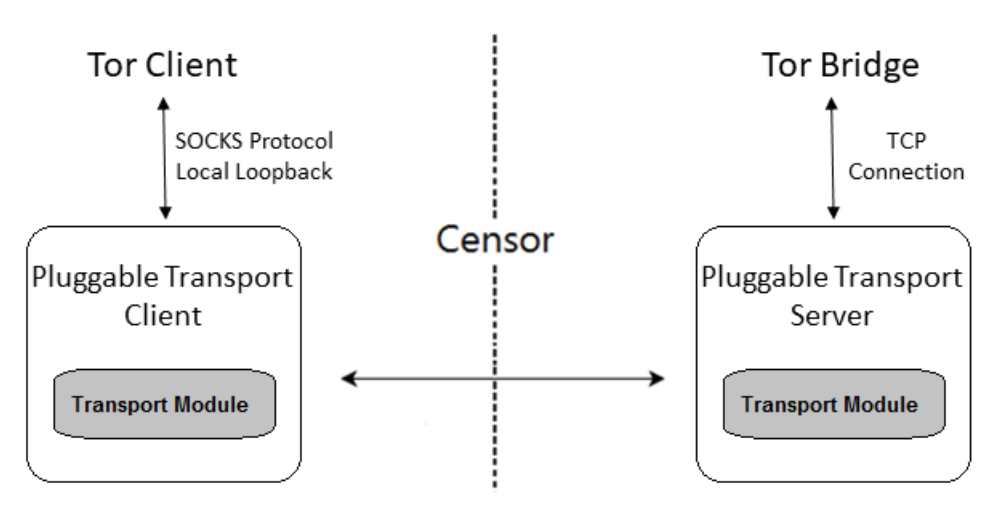
\includegraphics[width = 0.5\textwidth]{tor_pt.png}
        \caption{Схема Pluggable Transports}
        \label{spectrum}
    \end{center}
\end{figure}

PT представляют собой общую основу для разработки и развертывания технологий обхода блокировок.
Их основная задача - обфусцировать соединение между клиентом Tor и мостом, служащим защитой входа в Tor, так, чтобы оно выглядело доброкачественным.
PT состоит из двух частей, одна из которых устанавливается на стороне Tor-клиента, а другая - на стороне моста.
PT открывает SOCKS-прокси для клиентского приложения Tor, обфусцирует или иным образом преобразует трафик, прежде чем направить его на мост.
На стороне моста сервер PT выставляет обратный прокси, который принимает соединения от клиентов PT и декодирует обфускацию/трансформацию,
примененную к трафику, перед передачей его реальному приложению моста.
Данные, передаваемые между PT-клиентом и PT-сервером, могут быть зашифрованы, разрезаны на части общей длины или иным образом замаскированы,
что делает их труднодоступными для цензора, который может обнаружить данные Tor и заблокировать их.
Преобразование/обфускация данных и обратные операции выполняются транспортными модулями/протоколами обфускации, используемыми PT.
По состоянию на сентябрь 2017 года, доступными и развернутыми протоколами обфускации в браузере Tor являются: obfs3, obfs4, ScrambleSuit, FTE и meek.

\begin{enumerate}

    \item \textbf{Obfs3}: создает дополнительный уровень шифрования поверх TLS-соединения Tor, чтобы скрыть его уникальные характеристики.
    Для обмена ключами шифрования используется неаутентифицированный кастомизированное рукопожатие Диффи-Хеллмана.
    В результате этот протокол подвержен активным атакам на зондирование.

    \item \textbf{ScrambleSuit}: защищает от активных зондирующих атак, используя для аутентификации внеканальный обмен секретами и номерами сеансов.
    ScrambleSuit также способен изменять свой сетевой отпечаток (распределение длины пакетов, время между приходами и т.д.).
    Этот протокол является предшественником Obfs4 и подвержен цензуре на основе белых списков.

    \item \textbf{Obfs4}: имеет те же возможности, что и ScrambleSuit, но использует технику Elligator для обфускации открытых ключей
    и протокол ntor для односторонней аутентификации. В результате протокол работает быстрее, чем ScrambleSuit,
    и добавляет возможность мостовой аутентификации. Этот протокол также может быть заблокирован с помощью цензуры, основанной на белых списках.

    \item \textbf{Meek}: использует технику, называемую Domain Fronting, для ретрансляции Tor-трафика на Tor-мост через сторонние серверы
    (т.е. CDN, такие как Amazon CloudFront и Microsoft Azure).

    \item \textbf{Format-Transforming Encryption (FTE)}: преобразовывает трафик Tor в произвольные форматы стандартных протоколов, используя их языковые описания.

\end{enumerate}

Эти протоколы обфускации можно разделить на две группы:

\begin{enumerate}

    \item \textbf{Протоколы случайных потоков (obfs3, obfs4 и ScrambleSuit)}.
    Обмен данными в этих протоколах осуществляется в виде потоков случайных байтов,
    которые невозможно соотнести ни с одним известным протоколом.
    Эти протоколы состоят из двух фаз: фазы рукопожатия, на которой обе участвующие стороны надежно обмениваются ключами и/или номерами,
    и фазы коммуникации, состоящей в обмене зашифрованными сообщениями с использованием установленных ключей.

    \item \textbf{Структурированные потоковые протоколы (FTE и meek)},
    которые пытаются имитировать известные протоколы из ''белого списка'', такие как HTTP.

\end{enumerate}

Цензурирующие страны, обладающие возможностями активного зондирования, могут выявить мосты, взаимодействующие с использованием obfs3.
Кроме того, протоколы случайных потоков относятся к категории ''похожих на ничто'', что означает,
что они могут быть идентифицированы и заблокированы цензором с помощью стратегии ''белого списка'',
поскольку их отпечаток (включая рукопожатие) не соответствует ни одному известному протоколу.
C другой стороны, структурированные потоковые протоколы, имитирующие широко распространенные протоколы,
устойчивы к блокированию на основе ''белых списков''. Однако они не защищают от активного зондирования.

\section{FTE}

Часть DPI систем используют явно или неявно регулярные выражения для классификации протоколов на прикладном уровне,
поэтому рассмотрим механизмы, позволяющие злоумышленнику принудительно идентифицировать протокол, против любого DPI, основанного на проверке регулярных выражений.
Основная идея заключается в том, чтобы встроить защиту от DPI в схемы шифрования.
Добавим к обычному интерфейсу шифрования возможность принимать на вход регулярное выражение.
Задача этого регулярного выражения определять формат шифротекстов: это означает,
что шифротексты, взятые в виде строк соответствующего алфавита, гарантированно будут соответствовать заданному регулярному выражению.
Такой криптографический примитив называется форматно-преобразующим шифрованием.
Благодаря правильному выбору регулярного выражения, шифротексты, которые на самом деле несут исходный протокол,
будут классифицироваться DPI как сообщения от другого протокола, по нашему выбору.

Схема FTE состоит из трех алгоритмов: генерация ключа, шифрования и дешифрования.
Генерация ключа работает, как и в обычном шифровании, с выдачей случайно ывбранного симметричного ключа $K$.
Шифрование $Enc$ принимает ключ $\K$, формат $\F$ и сообщение $\M$.
Оно может быть случайным, полным или детерминированным и всегда выдаёт шифротекст $C$ или символ ошибки $\perp$.
Расшифрование $Dec$ принимает ключ $K$, формат $F$ и шифротекст $C$. Его выходом является сообщение или символ ошибки $\perp$.
Формат $F$ задаёт множество $L(F)$, называемое языком $F$.
Требование заключается в том, что любой шифротекст $С$, выводимый $Enc$, должен быть элементом $L(F)$.

FTE является схожим с шифрованием сохраняющий формат (FPE), впервые формализированного Bellare, Ristenpart, Rogaway и Stegers (BRRS).
В нём также используются форматы, но при этом требуется, чтобы и открытый текст, и шифротекст были элементами одного и того языка, определенного формата.

Хочется, чтобы FTE могло поддерживать форматы, описываемые регулярными выражениями.
Это легко позволит ''программировать'' форматы и наделит FTE теми выразительными возможностями, что и DPI системы, основанные на регулярных выражениях.

Реализация $Enc(K, F, M)$ для регулярного выражения $F$:
\begin{enumerate}
    \item Шифруем сообщение $M$ с помощью стандартной схемы аутентифицированного шифрования, получая промежуточный шифротекст $Y$.
    \item Рассматриваем $Y$ как число в $\mathbb{Z}_{|L(F)|}$ (в кольце класса вычетов по модулю размера языка).
\end{enumerate}


Применяем кодирующию функцию unrank: $\mathbb{Z}_{|L(F)|} \rightarrow L(F)$.
Для возможности расшифровки требуем, чтобы unrank была биективной функцией с эффективно вычислимой обратной функцией rank:  $L(F) \rightarrow \mathbb{Z}_{|L(F)|}$.
Ключевой алгоритмической проблемой является реализация функции rank и unrank эффективно.
Они связывают с каждой строкой языка её ранг, т.е. позицию в общем упоряченном языке.
Goldberg и Sipser предложили эффективный способ ранжирования регулярного языка, когда этот язык представлен детерминированным конечным автоматом (DFA).
BRRS использовали его для нереализованной схемы FPE для произвольных регулярных языков, закодированных как DFA, но они также подчеркивают,
что, асимптотически говоря, доказательно не существует способа дать эффективные функции rank и unrank, начиная с регулярных выражений.
Существует стандартные средства для преобразования регулярного выражения в недетерминированный конечный автомат (NFA),
а затем в DFA, но второй шаг приводит к экспоненциальному раздуванию размера состояния.
Такое поведение в худшем случае не является проблемой для FTE, отчасти потому,
что типы регулярных выражений, используемых в DPI, сами по себе явно разработаны для того, чтобы избежать раздувания в худшем случае.
Предложенная реализация использует компромисс между временем и памятью, предложенный Goldberg и Sipser,
для поддержки более эффективной работы во время выполнения программы путем предварительного вычисления таблиц,
позволяющих (не) ранжировать все строки $x \in L$, где $|x| \leq n$. Сложность таких предварительной обработки составляет $O(n \cdot |\Sigma| \cdot |Q|)$,
где $\Sigma$ - базовый алфавит, а $Q$ - множество состояний DFA, реализующего регулярное выражение FTE.
С учетом эти таблиц, сложность функций rankL и unrankL состовляет $\Omega(n)$ и $O(n · |\Sigma|)$, где n - длина выхода $rank_{L}$ и входа $unrank_{L}$ соответственно.
Подход ''Encrypt-then-Unrank'' сохраняет конфиденциальность сообщений и аутентичность базовой схемы аутентифицированного шифрования.


\section{DNS-Morph}
\section{Заключение}

\newpage

\begin{thebibliography}{9}
\bibitem {} Mihir Bellare, Thomas Ristenpart, Phillip Rogaway, Till Stegers. Format-Preserving Encryption.
\bibitem {} Kevin P. Dyer, Scott E. Coull, Thomas Ristenpart, Thomas Shrimpton. Protocol Misidentification Made Easy.
\bibitem {} Rami Ailabouni, Orr Dunkelman, Sara Bitan. DNS-Morph UDP-Based Bootstrapping Protocol For Tor.
\bibitem {} Piyush Sharma, Devashish Gosain. Camoufler Accessing The Censored Web By Utilizing Instant Messaging.
\bibitem {} Zhonghang Sui, Hui Shu, Fei Kang, Yuyao Huang, Guoyu Huo. A Comprehensive Review of Tunnel Detection on Multilayer Protocols.
\end{thebibliography}


\end{document}
